% Created 2018-05-17 Thu 16:07
% Intended LaTeX compiler: pdflatex
\documentclass[11pt]{article}
\usepackage[utf8]{inputenc}
\usepackage[T1]{fontenc}
\usepackage{graphicx}
\usepackage{grffile}
\usepackage{longtable}
\usepackage{wrapfig}
\usepackage{rotating}
\usepackage[normalem]{ulem}
\usepackage{amsmath}
\usepackage{textcomp}
\usepackage{amssymb}
\usepackage{capt-of}
\usepackage{hyperref}
\renewcommand{\thesection}{\Roman{section}}
\renewcommand{\thesubsection}{\thesection.\Roman{subsection}}
\renewcommand{\thesubsubsection}{\thesubsection.\Roman{subsubsection}}
\usepackage[parfill]{parskip}
\usepackage{color}
\usepackage{amsmath}
\usepackage{amssymb}
\usepackage{pgfplots}
\usepackage{mathtools}
\date{\today}
\title{}
\hypersetup{
 pdfauthor={},
 pdftitle={},
 pdfkeywords={},
 pdfsubject={},
 pdfcreator={Emacs 26.0.91 (Org mode 9.1.6)}, 
 pdflang={English}}
\begin{document}

\tableofcontents

\newpage

\section{Die kurze Frist}
\label{sec:org992bfd1}
\begin{itemize}
\item kombinierter Einsatz von Geld- und Fiskalpolitik\\
\end{itemize}

Zentrale Frage: \textbf{Wie hoch ist die Güterproduktion?}\\
-> Antworten aus der Keynesianischen Theorie:
\begin{itemize}
\item die Güterproduktion (Angebot) wird allein durch die Nachfrage bestimmt
\item angebotsseitige Einflüsse wie bswp Technologie und Qualifikation der Arbeitskräfte können vernachlässigt werden, weil die Nachfrage das Angebot nicht ausschöpft
\item Annahme dass Güterpreise konstant sind
\end{itemize}

Güternachfrage hängt von vielen Faktoren ab, u.a. vom \textbf{Gütermarkt} und dem Geschehen auf \textbf{Geld- und Finanzmärkten}. Im Folgenden daher Betrachtung von:
\begin{enumerate}
\item Gütermarkt
\begin{itemize}
\item Untersuchung des Gleichgewichts auf dem Gütermarkt
\item Beschreibung der \textbf{nachfrageseitigen} Bestimmung von Produktion und Einkommen
\item Analyse des Einflusses der Fiskalpolitik
\end{itemize}

\item Geld- und Finanzmärkte
\begin{itemize}
\item Untersuchung des Gleichgewichts auf den Geld- und Finanzmärkten
\item Beschreibung der Bestimmung des Zinses
\item Analyse des Einflusses der Geldpolitik
\end{itemize}

\item IS-LM-Modell
\begin{itemize}
\item Untersuchung des Zusammenwirkens von Güter-, Geld- und Finanzmärkten
\item Beschreibung der simultanen Bestimmung von Produktion \& Einkommen, sowie des Zinses
\begin{itemize}
\item dies bezeichnet man als IS-LM-Modell
\end{itemize}
\end{itemize}
\end{enumerate}

\subsection{Der Gütermarkt}
\label{sec:org76e20c7}
Markteilnehmer auf em Gütermarkt sind die volkswirtschaftl. Sektoren (Haushalte, Staat, Unternehmen)

\textbf{Makroökonomischer Gütermarkt=} (gedachte) Zusammenfassung aller Güterkäufe und -verkäufe in einem Land innerhalb 1 Periode (\(\approx\) BIP)

Angebot = inländische Produktion + Ausland(Import) = Y + IM

Nachfrage = Haushalte + Unternehmen + Staat + Ausland(Export) = C + I + G + X

Die Konsumausgaben (Nachfrage) der privaten Haushalte (C -> Consumers) entspricht allen Waren \& Dienstleistungen, die von Verbrauchern gekauft werden

Die Konsumausgaben (Nachfrage) des Staates (G -> Government) entspricht allen Waren \& Dienstleistungen, die durch den staatlichen Sektor (Bund, Länder und Gemeinden) gekauft werden.

Die Investitionen also die "Nachfrage" der Unternehmen (I) setzen sich zusammen aus Anlageinvestitionen (= gewerbliche Investitionen, Wohnungsbauinvestitionen) und Lagerinvestitionen (= Vorratsänderungen). Die Vorratsänderungen werden in unserem Modell zunächst vernachlässigt (Wert also gleich Null).
Die Investitionen lassen sich "brutto" (einschließlich Abschreibungen) und "netto" (ohne Abschreibungen) erfassen. Ergo entsprechen Bruttoinvestitionen = Nettoinvestitionen plus Abschreibungen. Abschreibungen vernachlässigen wir in diesem Modell jedoch auch zunächst (Wert gleich Null).

Die Exporte (X) entsprechen dem Kauf einheimischer Waren \& Dienstleistungen durch Ausländer.
Die Importe (IM) entsprechen dem Kauf ausländischer Waren \& Dienstleistungen durch einheimische Konsumenten, Unternehmen und staatl. Institutionen. Der Außenbeitrag (X-IM) entspricht der Differenz zwischen Exporten und Importen (= Nettoexporte):
\begin{itemize}
\item Exporte > Importe = positiver Außenbeitrag (Überschuss in Handels- und Dienstleistungsbilanz)
\item Exporte < Importe = negativer Außenbeitrag (Defizit in Handels- und Dienstleistungsbilanz)
\end{itemize}

\subsubsection{Die gesamtwirtschaftliche Güternachfrage}
\label{sec:org4c14213}
Ausgehend von der Zusammensetzung des Gütermarktes, also der Zusammenfassung aller Güterkäufe und -verkäufe, was wiederum etwa dem BIP entspricht, lässt sich die \textbf{Güternachfrage Z} wie folgt beschreiben: \(Z \equiv C + I + G + (X - IM)\). Dies ist zentral, da wir in der kurzen Frist ja den Fokus auf die Nachfrage und ihren Einfluss legen.
In einer geschlossenen Marktwirtschaft (keine Ex-/Importe) gilt dann: \(Z \equiv C + I+ G\).

\paragraph{Aufschlüsselung der Bestandteile von Güternachfrage Z}
\begin{enumerate}
\item Privater Konsum (C)
\label{sec:orge12e72e}
\begin{itemize}
\item Konsumentenverhalten wird durch \textbf{Konsumfunktion} C(Y\(_{\text{v}}\)) beschrieben
\item Konsum C steigt wenn verfügbares Einkommen Y\(_{\text{v}}\) zunimmt: \(C = C(Y_v) \rightarrow \frac{\partial C}{\partial Y_v} > 0\)
\item das verfügbare Einkommen Y\(_{\text{v}}\) entspricht dem Einkommen, was dem Verbraucher netto, d.h. \emph{nach Abzug der Steuern}  zur Verfügung steht: \(Y_v = Y - T\), wobei
\end{itemize}

Y\(_{\text{v}}\) = \emph{verfügbares} Einkommen,
Y = Einkommen,
T = Nettosteuern 

\begin{itemize}
\item es wird angenommen, dass diese Konsumfunktion C(Y\(_{\text{v}}\)) linear ist, also \(C = c_0 + c_1 * Y_v\) (keynesianische Konsumfunktion). Die Funktion hat zwei Parameter:
\begin{itemize}
\item c\(_{\text{1}}\) = \textbf{marginale Konsumneigung}, entspricht dem Effekt, den ein zusätzlicher Euro verfügbares Einkommen auf den Konsum hat (0 < c\(_{\text{1}}\) < 1)
\item c\(_{\text{0}}\) = \textbf{autonomer Konsum}, entspricht dem \textbf{autonomen Konsum} (c\(_{\text{0}}\) > 0), also wieviel konsumiert worden wäre selbst, wenn das Einkommen null wäre (Y-Achsenabschnitt)
\end{itemize}
\end{itemize}


\begin{equation*}
\begin{aligned}
& C = C(Y_v) = c_0 + c_1 * Y_v\\
& Y_v \equiv Y - T\\
& \rightarrow C = c_0 + c_1 * (Y - T) = c_0 + c_1  Y - c_1 T
\end{aligned}
\end{equation*}

Beispiel:

T = 0, 
c\(_{\text{0}}\) = 100,
c\(_{\text{1}}\) = 0.5,
T\(_{\text{1}}\) = 0

\(\rightarrow\) \textcolor{blue}{$C_1 = 100 + 0.5 * Y - 0.5 * 0$}

dann Einführung einer Steuer T = 50:\\
\(\rightarrow\) \textcolor{red}{$C_2 = 100 + 0.5 * Y - 0.5 * 50 = 75 + 0.5 * Y$}

Der Konsum beim Einkommen von Null (autonomer Konsum) sinkt durch die Besteuerung von 100 auf 75, aber die Steigung der Konsumfunktion (c\(_{\text{1}}\)) bleibt gleich:

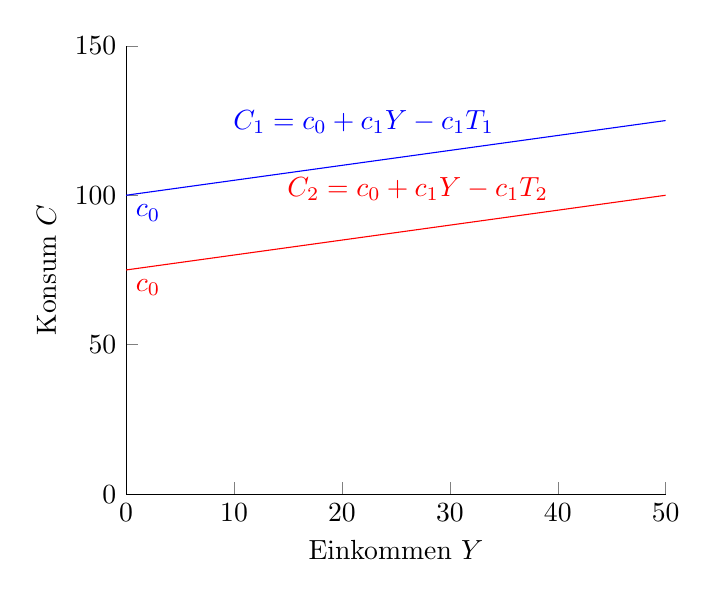
\begin{tikzpicture}
  \begin{axis}[ 
    xmin=0,   xmax=50,
    ymin=0,   ymax=150,
    domain=0:50,
    axis x line*=bottom,
    axis y line*=left,
    xlabel=$\text{Einkommen }Y$,
    ylabel={$\text{Konsum }C$}
  ] 
    \addplot +[mark=none] {100 + 0.5 * x}node[above left,pos=0.7] {$C_1 = c_0 + c_1 Y - c_1 T_1$} node[below right, pos=0] {$c_0$}; 
    \addplot +[mark=none] {75 + 0.5 * x}node[above left,pos=0.8] {$C_2 = c_0 + c_1 Y - c_1 T_2$} node[below right, pos=0] {$c_0$}; 
  \end{axis}
\end{tikzpicture}
\item Investitionen (I)
\label{sec:orge83954e}
\newline
Investitionen werden in diesem Modell als gegeben betrachtet, d.h als exogen angenommen. Gekennzeichnet wird dies durch einen Strich über der Variable: \(I = \bar{I}\) .
\item Staatsausgaben (G) und Steuern (T)
\label{sec:orgfc4169b}
\newline
Basierend auf dem Regierungsprogramm ergibt sich ein bestimmtes Ausmaß an Staatsausgaben und Steuern, in diesem Sinn sind beide ebenfalls exogen: \(G = \bar{G}\) und \(T = \bar{T}\) (T sind Steuern minus Transfers).

Laut Regierungsprogramm sind die Staatsausgaben durch Steuern finanziert, daher nehmen wir an, dass der Haushalt in der Ausgangssituation ausgeglichen ist: \(G = T\) .
Werden Staatsausgaben oder Steuern verändert, um die gesamtwirtschaftliche Nachfrage zu beeinflussen, spricht man von Fiskalpolitik
\end{enumerate}
\subsubsection{Gleichgewicht auf dem Gütermarkt (Bestimmung der Produktion)}
\label{sec:org6b95916}
Ein \textbf{Gleichgewicht auf dem Gütermarkt} stellt sich dann ein, wenn die \textbf{Güterproduktion Y} der \textbf{Güternachfrage Z} entspricht: \(Y = Z\). Dies ist eine Gleichgewichtsbedingung. Somit gilt (für \(X=IM=0\)):
\begin{equation*}
\begin{aligned}
Y = c_0 + c_1*(Y-\bar{T})+\bar{I}+\bar{G}
\end{aligned}
\end{equation*}
Im Gleichgewicht entspricht die Produktion Y (linke Seite) der Nachfrage (rechte Seite). Da Nachfrage < Produktionspotential, können die nachgefragten Güter auch produziert werden. Es gibt folgende Zusammenhänge:
\begin{itemize}
\item die Nachfrage (ergo dann = die Produktion, da Nachfrage in diesem Modell entscheidend ist) hängt ihrerseits vom Einkommen Y ab
\item das Einkommen Y wiederum ist gleich der Produktion (bzw dem Produktionswert) Y (weil jeder durch Produktion eingenommene Euro, als Einkommen eingenommen wurde)
\item somit wird dasselbe Symbol Y sowohl für die Produktion als auch fuer das Einkommen verwendet
\end{itemize}

Die Gleichgewichtsbedingung spiegelt die zentrale Modellannahme wieder, dass die Produktion nur durch die Nachfrage bestimmt wird (nachfrageseitiges Modell).

\subsubsection{Gleichungen des Gütermarktmodells}
\label{sec:org0a95c33}
Das Modell besteht aus folgenden Arten von Gleichungen:
\begin{itemize}
\item Definitionsgleichungen, hier: \(Z \equiv C + I + G\) und \(Y_v \equiv Y - T\)
\item Verhaltensgleichungen, hier: \(C= c_0 + c_1*(Y-T)\)
\item Gleichgewichtsbedingung, hier: \(Y=Z\) (Produktion = Güternachfrage)
\end{itemize}

Die Modellgleichungen enthalten:
\begin{itemize}
\item endogene Variablen, hier: C, Y, Z
\item exogene Variablen, hier: \(\bar{I}, \bar{G}, \bar{T}\)
\item Parameter, hier: c\(_{\text{0}}\), c\(_{\text{1}}\)
\end{itemize}

In Modellen analysieren wir meist nur gleichgewichtige Situationen.

Die Gleichgewichtsbedingung kann unter Einführung zwei neuer Begriffe wiefolgt umformuliert werden:

\begin{equation*}
\begin{aligned}
Y = c_0 + c_1*(Y-\bar{T})+\bar{I}+\bar{G}\\
Y = c_0 + c_1*Y - c_1 * \bar{T}+\bar{I}+\bar{G} & \qquad |-(c_1*Y) \nonumber\\
Y - c_1 * Y = c_0 - c_1 * \bar{T}+\bar{I}+\bar{G}\\
(1 - c_1)* Y = c_0 - c_1 * \bar{T}+\bar{I}+\bar{G}  & \qquad |:(1-c_1) \nonumber\\
Y = \frac{c_0 - c_1 * \bar{T}+\bar{I}+\bar{G}}{1-c_1} & \qquad | \text{aus Bruch vorziehen}\\
Y = \frac{1}{1-c_1}*[c_0 - c_1 * \bar{T}+\bar{I}+\bar{G}]
\end{aligned}
\end{equation*}
\begin{itemize}
\item \(\frac{1}{1-c_1}\) = Multiplikator
\item \([c_0 - c_1 * \bar{T}+\bar{I}+\bar{G}]\) = autonome Ausgaben
\end{itemize}

\subsubsection{Graphische Analyse}
\label{sec:org1b4350a}
\(\rightarrow\) Siehe handschriftliches Blatt

\subsubsection{Der Multiplikatoreffekt}
\label{sec:orgfe9da55}
Der Multiplikator ist die Summe sukzessiver Anstiege der Produktion, die aus einem Anstieg der Nachfrage resultieren

Beispielsweise eine Erhöhung der autonomen Staatsausgaben: \(\Delta Y_1 = \Delta \bar{G}\)

\begin{enumerate}
\item Folgerunde: Erhöhung des Konsums: \(\Delta Y_2 = \Delta C_1 = c_1 * \Delta Y_1 = c_1*\Delta \bar{G}\)

\item Folgerunde: Erhöhung des Konsums: \(\Delta Y_3 = \Delta C_2 = c_{1}^{2} * \Delta Y_2 = c_{1}^{2} *\Delta \bar{G}\)
\end{enumerate}

..es folgen weitere Runden, insgesamt ergibt sich: Anstoß + induzierte Konsumnachfrage

Steigt die autonome Nachfrage um 1 Mio., dann ergibt sich nach \(n\) Runden eine Erhöhung der Produktion um 1 Mio. \emph{multipliziert} mit der folgenden Summe: \(1+ c_1 + c_{1}^{2} + ... + c_{1}^{n}\). Das ist eine geometrische Reihe für die bei \(c_1<1\) gilt:

\begin{equation*}
\begin{aligned}
\lim\limits_{n \to \infty}1+ c_1 + c_{1}^{2} + c_{1}^{3} + ... + c_{1}^{n} = \frac{1}{1-c_1}\
\end{aligned}
\end{equation*}

\subsubsection{Die verbale Analyse}
\label{sec:orgf4c848e}
Kurzfristig (in der kurzen Frist) wird die Produktion von der Nachfrage bestimmt
\begin{itemize}
\item die Nachfrage hängt ihrerseitz vom Einkommen ab Z(Y)
\end{itemize}

Ein Anstieg der Nachfrage (zB Anstieg der Staatsausgaben) führt zu Anstieg der Produktion und zu einem entsprechenden Anstieg des Einkommens
\begin{itemize}
\item diese Einkommenserhöhung induziert einen weiteren Anstieg der Nachfrage \(\rightarrow\) dies führt wiederum zu einer weiteren Produktionssteigerung usw.
\end{itemize}

Im Endergebnis fällt der Anstieg weit größer aus als die ursprüngliche Verschiebung der Nachfrage und zwar genau um den Faktor, der dem Multiplikator entspricht

Wie lange dauert es bis dieser Anpassungsprozess abgeschlossen ist?
Nach einem Anstieg der Konsumausgaben wird nicht sofort das neue Gleichgewicht erreicht. Es findet vielmehr ein allmählicher Prozess der Anpassung statt.
\begin{itemize}
\item Geschwindigkeit hängt davon ab wie schnell die Firmen auf die neue Situation mit Produktionsanpassungen reagieren
\end{itemize}

Die formale Beschreibung dieser Anpassung der Produktion über die Zeit wird als \textbf{Dynamik} der Anpassung bezeichnet.

\subsubsection{Investition gleich Ersparnis}
\label{sec:org5d1b42c}
Rest des verfügbaren Einkommens, der nicht für Konsum ausgegeben wird, wird gespart:

\begin{itemize}
\item Definitionsgleichung, hier: \(S = Y_v - C\)
\item Verhaltensgleichung (keynesianische Sparfunktion), hier:
\end{itemize}
\begin{equation*}
\begin{aligned}
S = Y - T - c_0 - c_1(Y-T) \\
= -c_0 + (1-c_1)*(Y-T)
= -c_0 + (1-c_1) * Y_v
\end{aligned}
\end{equation*}
\begin{itemize}
\item Gleichgewichtsbedingung, hier:
\end{itemize}
\begin{equation*}
\begin{aligned}
Y = C + I + G
Y - T -C = I + G - T
S = I + G - T
I = S + (G-T)
\end{aligned}
\end{equation*}
S = Ersparnis privater Haushalte, (T - G) = Ersparnis des Staates

\subsubsection{Ist die Regierung allmächtig? Eine Warnung}
\label{sec:org1c6fcc6}
\begin{enumerate}
\item Kann die Regierung Einfluss nehmen?
\label{sec:org6f6deed}

Fiskalpolitik = Teil der Finanzpolitik, der dem Stabilisierungsziel gewidmet ist; die Variation von Staatsausgaben bzw -einnahmen zur Beeinflussung der aggregierten Güternachfrage
\begin{center}
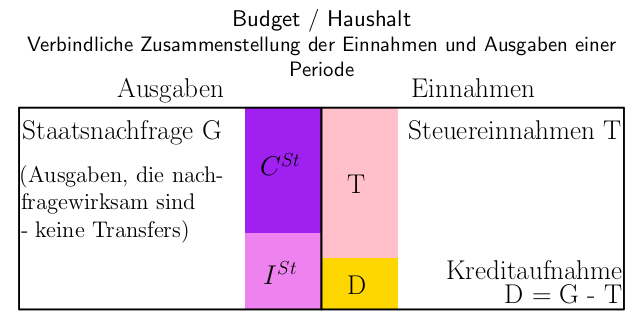
\includegraphics[width=.9\linewidth]{./budgethaushalt.png}
\end{center}

\(Y = \frac{1}{1-c_1}*[c_0-c_1\textcolor{magenta}{\bar{T}} + \bar{I} + \textcolor{magenta}{\bar{G}}]\)

direkte Maßnahmen:
\begin{itemize}
\item Änderung der Staatsausgaben
\item Änderung der Steuern bzw der Transfers
\end{itemize}

indirekte Maßnahmen:
\begin{itemize}
\item Investitionszulagen
\item Abschreibungsvergünstigungen
\end{itemize}

\item Wer ist für Fiskalpolitik verantwortlich?
\label{sec:org96819c3}

Staat = Institution mit hoheitlicher Gewalt, d.h. Staat ist legitimiert \& fähig Zwangsmaßnahmen auszuüben

Staatsquote = \(\frac{\text{Ausgaben der öffentl. Haushalte}}{\text{Bruttoinlandsprodukt}}\) in Prozent
\item Kreditfinanzierte Erhöhung der Staatsausgaben
\label{sec:org8ddfa50}

Eine Erhöhung der Staatsausgaben G erhöht die Nachfrage (\(\rightarrow\) Z-Kurve verschiebt sich nach oben), sodass Einkommen steigt und zwar gemäß dem Multiplikator um \(\frac{\delta Y}{\delta G} = \frac{1}{1-c_1}\).

Da die zusätzlichen Ausgaben kreditfinanziert werden, wird die staatliche Ersparnis (T - G) kleiner. Dies wird aber durch die private Ersparnis S ausgeglichen, die mit dem Einkommen ansteigt.

Da die erhöhten Staatsausgaben kreditfinanziert werden, vergrößert sich der Schuldenstand des Staates (nicht in unserem Modell enthalten!).
\item Steuerfinanzierte Erhöhung der Staatsausgaben
\label{sec:orgfad82e1}

Eine Erhöhung der Staatsausgaben G wird durch eine gleichzeitige Erhöhung der Steuern T finanziert:
\begin{equation*}
\begin{aligned}
Y = \frac{1}{1-c_1}*[c_0-c_1*\bar{T}+\bar{I}+\bar{G}]\\
Y = \frac{1}{1-c_1}*[c_0+\bar{I}+(1 - c_1)*\bar{G}]
\end{aligned}
\end{equation*}
Auch in der neuen Situation gilt G = T und damit bei steuerfinanzierten Änderungen von G: \(\frac{\delta Y}{\delta G} = \frac{1-c_1}{1-c_1} = 1\).
Der Multiplikator ist somit lediglich 1 und damit kleiner als bei kreditfinanzierten Staatsausgaben. Das ergibt sich auch bei separater Betrachtung der Multiplikatoren:
\begin{equation*}
\begin{aligned}
{\underbrace{\textstyle \frac{1}{1-c_1}}_{\mathclap{\text{ Staatsausgabenmultiplikator }}}} 
+
{\overbrace{\textstyle \frac{-c_1}{1-c_1}}^{\mathclap{\text{ Steuermultiplikator }}}}
=
1
\end{aligned}
\end{equation*}

\item Automatische Stabilisatoren
\label{sec:org9935559}

Idee: Konjunkturelle Schwankungen der Steuereinnahmen stabilisieren Nachfrage \(Z = c_0 + c_1 *(Y-T)+\bar{I}+\bar{G}\). Steuern (und Transfers) hängen endogen vom Einkommen ab: \(T= t*Y\), mit \(t=\text{Steuersatz} < 1\)

\begin{equation*}
\begin{aligned}
Y = Z = c_0 + c_1- c_1  t Y + \bar{I} + \bar{G} & \qquad |+(c_1*t*Y),|-c_1 \nonumber\\
Y - c_1 + c_1*t*Y = c_0 + \bar{I} + \bar{G}\\
Y (1-c_1+c_1t) = c_0 + \bar{O} + \bar{G}\\
Y = \frac{1}{1-c_1+c_1t}*[c_0+\bar{I}+\bar{G}]
\end{aligned}
\end{equation*}

Der Multiplikator wird kleiner. Bei exogenen Schocks in \(\bar{I}\) oder c\(_{\text{o}}\) fallen Schwankungen geringer aus.

\item Probleme bei Umsetzung direkter Nachfragesteuerung
\label{sec:org7581194}

\begin{itemize}
\item Staatsausgaben oder Steuern rasch zu ändern ist nahezu unmöglich
\item aufgrund komplexer Prozesse sind Auswirkungen auf Konsum, Investitionen, Importe etc. nur mit großer Unsicherheit zu prognostizieren
\item Erwartungen spielen eine große Rolle
\item empirisch ermittelte Multiplikatoren sind viel kleiner als im Modell und teilweise sogar < 1
\item das Ziel eines bestimmten Produktionsniveaus kann unerwünschte Nebenwirkungen nach sich ziehen (zB Preissteigerungen)
\item ein hohes Budgetdefizit \& hohe Staatsverschuldung kann langfristig schädliche Effekte auslösen
\end{itemize}
\end{enumerate}

\subsection{Geld- und Finanzmärkte}
\label{sec:org72c0576}
In diesem Kapitel geht es um das \textbf{Gleichgewicht} auf \textbf{Geld-} und \textbf{Finanzmärkten} und die \textbf{Bestimmung des Zinssatzes}.

\textbf{Geld} kann für Transaktionen (zB Kauf/Verkauf) verwendet werden. Es gibt zwei Arten von Geld:
\begin{itemize}
\item Bargeld (Münzen und Banknoten)
\item Sichtguthaben (Girokonten)
\end{itemize}

Geld kann auch zur Wertaufbewahrung verwendet werden. Da es aber keine Zinsen bringt, werden meist andere Formen der Wertaufbewahrung vorgezogen.

\textbf{Festverzinsliche Wertpapiere} (Bonds) bringen einen positiven Zinssatz i, können aber nicht für Transaktionen verwendet werden.

\textbf{Semantische Fallen:} Geld, Einkommen und Vermögen
\begin{itemize}
\item Einkommen besteht aus der Arbeitsvergütung \& Kapitalerträgen in Form von Zinsen \& Dividenden.
\begin{itemize}
\item wird in Einheiten pro Zeiteinheit ausgedrückt, es handelt sich also um eine Stromgröße
\end{itemize}
\item Ersparnis ist der Teil des Einkommens nach Abzug der Steuern, der nicht ausgegeben wird
\begin{itemize}
\item ebenfalls eine Stromgröße
\end{itemize}
\item Finanzvermögen (oder einfach Vermögen) ist Wert aller Finanzanlagen abzüglich aller Verbindlichkeiten
\begin{itemize}
\item Bestand an Vermögen zu einem gegebenen Zeitpunkt, also eine Bestandsgröße
\end{itemize}
\item Finanzanlagen, die man direkt zum Kauf von Gütern einsetzen kann, werden Geld genannt
\begin{itemize}
\item Geld beinhaltet Bargeld \& Buchgeld (Sichteinlagen)
\item ist auch eine Bestandsgröße
\end{itemize}
\item unter Investitionen verstehen Ökonomen den Kauf von neuen Anlagegütern (Maschinen, Fabriken, Bürogebäude), der Kauf von Aktien oder anderer Finanzanlagen wird dagegen als Finanzinvestition bezeichnet
\end{itemize}

Das Finanzvermögen W der Haushalte setzt sich zusammen aus Geldvermögen und Bonds. Geld wird i.d.R durch das Symbol M gekennzeichnet, Bonds(B) ist der Bestand an festverzinslichen Wertpapieren. Sie habenn den Preis p\(_{\text{B}}\) .
\begin{equation*}
\begin{aligned}
W = M + p_B * B
\end{aligned}
\end{equation*}
Haushalte haben darüber zu entscheiden, welchen Teil ihres Vermögens sie in Form von Geld und welchen in Form von Bonds halten. Geld hat den Vorteil der Liquidität, Bonds den eines Zinsertrages. Die Aufteilung ist abhängig von Transaktionsvolumen und -häufigkeit, sowie dem Zinssatz auf Wertpapiere
\subsubsection{Die Geldnachfrage}
\label{sec:orgb1328f1}
Die Geldnachfrage M\(^{\text{d}}\)\ldots{}
\begin{itemize}
\item \ldots{}steigt proportional mit dem Nominaleinkommen (\(PY\))
\item hängt negativ vom Zinssatz i ab (wobei L(i) eine Funktion des Zinssatzes ist)
\end{itemize}
\begin{equation*}
\begin{aligned}
M^d = PY*L(i)
\end{aligned}
\end{equation*}
\end{document}
